\documentclass[lang=cn,11pt,a4paper,cite=authornum]{paper}

\title{编译原理与技术 实验三:语法分析程序的设计与实现 \\ 实验报告}
\author{毛子恒 \\ 2019211397}
\institute{北京邮电大学\ 计算机学院}

\date{\zhtoday}

% 本文档命令
\usepackage{array}
\newcommand{\ccr}[1]{\makecell{{\color{#1}\rule{1cm}{1cm}}}}
\nocite{*}

\begin{document}

\maketitle

\section{概览}

\subsection{任务描述}

编写语法分析程序,实现对算术表达式的语法分析。要求所分析算术表达式由如下的文法产生。

\label{grammar}
$$
    \begin{aligned}
         & E\rightarrow E+T | E-T | T \\
         & T\rightarrow T*F | T/F | F \\
         & F\rightarrow (E) | num
    \end{aligned}
$$

要求在对输入的算术表达式进行分析的过程中,依次输出所采用的产生式。

编写语法分析程序实现自底向上的分析,要求如下:

\begin{enumerate}
    \item 构造识别该文法所有活前缀的DFA。
    \item 构造该文法的LR分析表。
    \item 构造LR分析程序。
\end{enumerate}

\subsection{开发环境}

\begin{itemize}
    \item macOS Big Sur 11.6.1
    \item Apple clang version 12.0.5
    \item cmake version 3.20.3
    \item Clion 2021.2.1
    \item Visual Studio Code 1.62.3
\end{itemize}

\section{模块介绍}

\subsection{模块划分}

各模块及其关系如\figref{fig:structure}。

\begin{figure}[htbp]

    \centering
    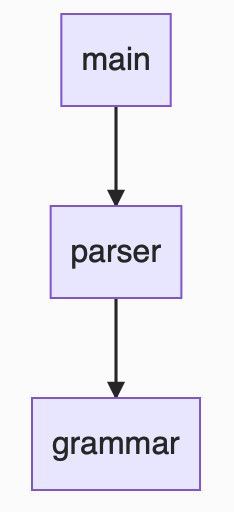
\includegraphics[width=0.15\linewidth]{./images/structure.png}
    \caption{模块关系图\label{fig:structure}}

\end{figure}

其中,\mintinline{text}{grammar}模块定义了文法类,其中实现了文法的输入、拓广文法、构建LR(1)项目集规范族及识别所有活前缀DFA的算法;\mintinline{text}{parser}模块定义了LR预测分析类,实现了从LR(1)项目集规范族及识别所有活前缀的DFA构造LR(1)分析表的算法,以及LR分析算法。

主函数的流程如下:

\begin{itemize}
    \item 从文件中读入文法。
    \item 构造LR(1)项目集规范族及识别所有活前缀的DFA并且判断是否是LR(1)文法。
    \item 利用DFA构建预测分析表。
    \item 从文件中读入需要分析的字符串。
    \item 对字符串进行LR分析,输出分析过程。
\end{itemize}

\subsection{文法类}

\mintinline{text}{grammar}模块中定义了LR(1)文法类:

\begin{code}
    \begin{minted}{C++}
using Symbol = std::string;
using SymbolSet = std::unordered_set<Symbol>;
using ProductionRight = std::deque<std::string>;
using Production = std::pair<Symbol, ProductionRight>;
using Productions = std::unordered_map<Symbol, std::vector<Production>>;
using Item = std::pair<const Production *, ProductionRight::const_iterator>;
extern const std::string EMPTY;
struct ItemSet
{
    std::map<Item, SymbolSet> shift_item;
    std::map<Item, SymbolSet> reduce_item;
    bool operator==(const ItemSet &rhs);
};
struct DFA
{
    std::vector<ItemSet *> states;
    std::vector<std::unordered_map<Symbol, int>> next;
};
class Grammar
{
public:
    Grammar() = default;
    void LoadFromFile(std::ifstream &fs);
    bool ConstructLR1StateMachine();
    const Symbol &GetStart() const;
    const SymbolSet &GetTerminal() const;
    const DFA &GetDfa() const;
private:
    SymbolSet nonterminal;
    SymbolSet terminal;
    Productions productions;
    Symbol start;
    std::unordered_map<Symbol, SymbolSet> first;
    std::map<Item, SymbolSet> item_first;
    DFA dfa;
    void Closure(ItemSet &item_set);
    void ConstructFirst(const Symbol &left);
    void ConstructItemFirst();
    void ExtendGrammar();
    void ConstructDFA();
    bool IsLR1Grammar() const;
};
template<typename T>
bool InSet(const std::unordered_set<T> &a, const T &b);
template<typename T1, typename T2>
bool InSet(const std::unordered_map<T1, T2> &a, const T1 &b);
std::ostream &operator<<(std::ostream &os, const SymbolSet &rhs);
std::ostream &operator<<(std::ostream &os, const ProductionRight &rhs);
std::ostream &operator<<(std::ostream &os, const Production &rhs);
std::ostream &operator<<(std::ostream &os, const Productions &rhs);
std::ostream &operator<<(std::ostream &os, const Item &rhs);
std::ostream &operator<<(std::ostream &os, const ItemSet &rhs);
std::ostream &operator<<(std::ostream &os, const DFA &rhs);
\end{minted}
\end{code}

\mintinline{text}{ProductionRight}类型表示产生式的右部,\mintinline{text}{Production}类型表示产生式,\mintinline{text}{Item}类型表示一个LR(0)项目(即不包含向前看符号集);\mintinline{text}{ItemSet}类型表示一个LR(1)项目集,其中分别有移进/待约项目和归约项目;\mintinline{text}{DFA}类型表示一个识别所有活前缀的DFA。

\mintinline{text}{Grammar}类中包含有文法的非终结符号集合、终结符号集合、产生式集合、起始符号、非终结符的FIRST集合、待约项目的FIRST集合。

\subsubsection{文法的输入}

\mintinline{text}{LoadFromFile}方法实现了从一个文件输入流中读取文法,一个描述\ref{grammar}节中文法的文件示例如下:

\label{grammar_text}
\begin{code}
    \begin{minted}{text}
$ Nonterminal symbols
E T F
$ Terminal symbols
+ - * / ( ) num
$ Start symbol
E
$ Productions
E -> E + T $ E - T $ T
T -> T * F $ T / F $ F
F -> ( E ) $ num
\end{minted}
\end{code}

文件依次输入非终结符号集合、终结符号集合、起始符号、文法产生式集合。每个部分的开始都以一行单独的说明字符串标识,各个部分均可包含多行,各个符号之间以空格分隔。产生式中以\mintinline{text}{$}符号代替\mintinline{text}{|}符号。

输入时,程序会对文法的合法性进行基本的判断,包括非终结符号集和终结符号集不重合、起始符号是非终结符号、产生式左部是非终结符号、右部是非终结符号或者终结符号。

\subsubsection{构造LR(1)项目集规范族及识别所有活前缀的DFA}

\mintinline{text}{ConstructLR1StateMachine}方法实现了构造LR(1)项目集规范族及识别所有活前缀的DFA,该方法依次调用\mintinline{text}{ExtendGrammar}、\mintinline{text}{ConstructItemFirst}、\mintinline{text}{ConstructDFA}、\mintinline{text}{IsLR1Grammar}方法,并在这期间输出调试信息。

\paragraph{拓广文法} \mintinline{text}{ExtendGrammar}方法实现了拓广文法,即对于文法$G=(N,T,P,S)$,生成与其等价的文法$G'=(N\cup \{S'\},T,P\cup\{S'\rightarrow S\},S')$。

\paragraph{构建非终结符和待约项目的FIRST集} \mintinline{text}{ConstructItemFirst}方法实现了构建非终结符和移进项目的FIRST集。

对于任意产生式$A\rightarrow\alpha$,若$\alpha\not=\varepsilon$,设该产生式为:

$$
    A\rightarrow Y_1Y_2\ldots Y_k
$$

遍历产生式右部的每一个$Y_i$,如果:

\begin{itemize}
    \item $Y_i$是终结符,则$\alpha$的FIRST集中增加$Y_i$,终止遍历;
    \item $Y_i$是非终结符,如果没有求出它的FIRST集,则递归求解。之后,$\alpha$的FIRST集并上$Y_i$的FIRST集。此后检查$Y_i$的FIRST集中是否包含$\varepsilon$(即是否能推导出$\varepsilon$),若不包含,则终止遍历。
\end{itemize}

最后,$A$的FIRST集为各个候选式的FIRST集的并。

对于每一个待约项目$A\rightarrow\alpha B\beta$,需要求出$\beta$的FIRST集,方法类似。

该算法的伪代码见\algoref{algo:cons_first}。

\begin{algorithm}[!htbp]
    \caption{构建非终结符和待约项目的FIRST集\label{algo:cons_first}}
    \KwIn{$\mathbf G = (\mathbf N, \mathbf T, \mathbf P, S)$}
    \KwOut{$\mathbf{FIRST}$}
    \SetKwProg{Fn}{Function}{}{end}
    \SetKwData{P}{$\mathbf P$}
    \SetKwData{N}{$\mathbf N$}
    \SetKwData{T}{$\mathbf T$}
    \SetKwData{FIRST}{$\mathbf{FIRST}$}
    \SetKwFunction{ConsFirst}{ConstructFirst}
    \SetKwFunction{ConsFirstSet}{ConstructItemFirst}
    \Fn(){\ConsFirst{A}}{
        \ForEach{$A\rightarrow\alpha\in\P$}{
            \If{$\alpha=\varepsilon$}{
                $\FIRST(A)\leftarrow\FIRST(A)\cup\{\varepsilon\}$\;
                $\FIRST(\alpha)\leftarrow\{\varepsilon\}$\;
            }
            \For(\tcp*[f]{$\alpha=Y_1Y_2\ldots Y_k$}){$i\leftarrow 1$ \KwTo $k$}{
                \If{$Y_i\in\T$}{
                    $\FIRST(\alpha)\leftarrow\FIRST(\alpha)\cup\{Y_i\}$\;
                    break\;
                }
                \lIf{$\FIRST(Y_i)=\varnothing$}{\ConsFirst{$Y_i$}}
                $\FIRST(\alpha)=\FIRST(\alpha)\cup\FIRST(Y_i)$\;
                \lIf{$\varepsilon\not\in\FIRST(Y_i)$}{break}
            }
            \lIf{$i=k$}{$\FIRST(A)\leftarrow\FIRST(A)\cup\{\varepsilon\}$}
            $\FIRST(A)\leftarrow\FIRST(A)\cup\FIRST(\alpha)$\;
        }
    }
    \Fn(){\ConsFirstSet{}}{
        \ForEach{$A\rightarrow\alpha\in\P$}{
            \For(\tcp*[f]{$\alpha=Y_1Y_2\ldots Y_k$}){$i\leftarrow 1$ \KwTo $k$}{
                \If{$Y_i\in\N$}{
                    \For(\tcp*[f]{$\beta=Y_{i+1}\ldots Y_k$}){$j\leftarrow i+1$ \KwTo $k$}{
                        \If{$Y_j\in\T$}{
                            $\FIRST(\beta)\leftarrow\FIRST(\beta)\cup\{Y_j\}$\;
                            break\;
                        }
                        \lIf{$\FIRST(Y_j)=\varnothing$}{\ConsFirst{$Y_j$}}
                        $\FIRST(\beta)=\FIRST(\beta)\cup\FIRST(Y_i)$\;
                        \lIf{$\varepsilon\not\in\FIRST(Y_j)$}{break}
                    }
                }
            }
        }
    }
\end{algorithm}

\paragraph{构造LR(1)项目集的闭包} \mintinline{text}{Closure}方法构造一个LR(1)项目集$I$的闭包$closure(I)$,构造方法如下:

\begin{enumerate}
    \item 初始化$closure(I)\leftarrow I$;
    \item 对于$[A\rightarrow \alpha\cdot B\beta, a]\in closure(I)$,若$B\rightarrow\eta\in \mathrm P$,则$\forall b\in FIRST(\beta a)$,使$closure(I)\leftarrow closure(I)\cup [B\rightarrow \cdot \eta,b]$;
    \item 重复2直至$closure(I)$不再增大为止。
\end{enumerate}

该算法的伪代码见\algoref{algo:closure}。

\begin{algorithm}[!htb]
    \caption{构造LR(1)项目集的闭包\label{algo:closure}}
    \KwIn{$\mathbf G = (\mathbf N, \mathbf T, \mathbf P, S),\mathbf I,\mathbf{FIRST}$}
    \KwOut{$\mathbf J=closure(\mathbf I)$}
    \SetKwProg{Fn}{Function}{}{end}
    \SetKwData{P}{$\mathbf P$}
    \SetKwData{N}{$\mathbf N$}
    \SetKwData{I}{$\mathbf I$}
    \SetKwData{J}{$\mathbf J$}
    \SetKwData{nJ}{$\mathbf{J'}$}
    \SetKwData{FIRST}{$\mathbf{FIRST}$}
    \SetKwFunction{Closure}{Closure}
    \Fn(){\Closure{\I}}{
        $\J\leftarrow\I$\;
        \Do{true}{
            $\nJ\leftarrow\J$\;
            \ForEach{$[A\rightarrow \alpha\cdot B\beta, a]\in\J$}{
                \ForEach{$B\rightarrow\eta\in\P$}{
                    \lForEach{$b\in(\FIRST(\beta)-\varepsilon)$}{$\nJ\leftarrow[B\rightarrow \cdot \eta,b]$}
                    \lIf{$\varepsilon\in\FIRST(\beta)$}{$\nJ\leftarrow[B\rightarrow \cdot \eta,a]$}
                }
            }
            \lIf{$\nJ=\J$}{break}
            $\J\leftarrow\nJ$\;
        }
    }
\end{algorithm}

\paragraph{构造LR(1)项目集规范族} \mintinline{text}{ConstructDFA}方法构造LR(1)文法的项目集规范族和识别所有活前缀的DFA。

该算法通过广度优先搜索求出识别所有活前缀的DFA。该算法的伪代码见\algoref{algo:dfa}。

\begin{algorithm}[!htbp]
    \caption{构造LR(1)项目集规范族\label{algo:dfa}}
    \KwIn{$\mathbf G = (\mathbf N, \mathbf T, \mathbf P, S),\mathbf{FIRST}$}
    \KwOut{$\mathbf M = (\mathbf N\cup \mathbf T, \mathbf Q, \mathbf I_0, \mathbf F=\mathbf Q, \delta)$}
    \SetKwProg{Fn}{Function}{}{end}
    \SetKwData{N}{$\mathbf N$}
    \SetKwData{T}{$\mathbf T$}
    \SetKwData{I}{$\mathbf I$}
    \SetKwData{J}{$\mathbf J$}
    \SetKwData{Q}{$\mathbf Q$}
    \SetKwData{tot}{total}
    \SetKwData{q}{queue}
    \SetKwData{go}{go}
    \SetKwFunction{Push}{push}
    \SetKwFunction{Pop}{pop}
    \SetKwFunction{Front}{front}
    \SetKwFunction{Emp}{empty}
    \SetKwFunction{ConsDFA}{ConstructDFA}
    \Fn(){\ConsDFA{\I}}{
    $\I_0\leftarrow\Closure{$\{[S'\rightarrow\cdot S,\$]\}$}$\;
    $\Q\leftarrow \Q\cup\{\I_0\}$\;
    $\q.\Push(\I_0)$\;
    $\tot\leftarrow0$\;
    \While{$\q.\Emp()$}{
    $\I_i\leftarrow\q.\Front()$\;
    $\q.\Pop()$\;
    \ForEach{$X\in\N\cup\T$}{
    $\go(\I_i,X)\leftarrow\Closure{$\{[A\rightarrow\alpha X\cdot\beta,a]|[A\rightarrow\alpha\cdot X\beta,a]\in\I_i\}$}$\;
    \If{$\go(\I_i,X)\not=\varnothing$}{
        \If{$\go(\I_i,X)\not\in\Q$}{
            $\tot\leftarrow\tot+1$\;
            $\I_{\tot}\leftarrow\go(\I_i,X)$\;
            $\Q\leftarrow\Q\cup\{\I_{\tot}\}$\;
            $\delta(\I_i,X)\leftarrow\I_{\tot}$\;
            $\q.\Push(\I_{\tot})$\;
        }
        \Else(\tcp*[f]{$\I_j=\go(\I_i,X)$}){
            $\delta(\I_i,X)\leftarrow\I_j$\;
        }
    }
    }
    }
    }
\end{algorithm}

\paragraph{判断是否是LR(1)文法} \mintinline{text}{IsLR1Grammar}方法判断文法是否是LR(1)文法,即检查每个项目集$\mathbf I$,要求其中任意两个归约项目的向前看符号集合交集为空,任意一个归约项目向前看符号集合和移进项目的移进符号集合交集为空。

\subsection{LR分析}

\mintinline{text}{parser}模块定义了LR分析类:

\begin{code}
    \begin{minted}{C++}
class Parser
{
public:
    Parser() = default;
    explicit Parser(const Grammar &grammar);
    bool ParseString(const ProductionRight &str);
private:
    using Status = std::pair<std::pair<std::vector<int>, std::vector<Symbol>>, ProductionRight>;
    enum ActionClass;
    struct ActionItem
    {
        ActionClass action_class;
        union
        {
            int index;
            const Production * production;
        };
    };
    SymbolSet terminal;
    std::vector<std::unordered_map<Symbol, ActionItem>> action_table;
    std::vector<std::unordered_map<Symbol, int>> goto_table;
    int NextStep(Status &status) const;
    friend std::ostream &operator<<(std::ostream &os, const Parser &rhs);
    friend std::ostream &operator<<(std::ostream &os, const ActionItem &action_item);
};
std::ostream &operator<<(std::ostream &os, const std::pair<std::vector<int>, std::vector<Symbol>> &rhs);
\end{minted}
\end{code}

\subsubsection{构建LR分析表}

\mintinline{text}{Parser(const Grammar &grammar)}构造函数通过LR(1)项目集规范族构造一个LR分析表,构造算法伪代码见\algoref{algo:cons_table}。

\begin{algorithm}[!htb]
    \caption{构建LR分析表\label{algo:cons_table}}
    \KwIn{$\mathbf G = (\mathbf N, \mathbf T, \mathbf P, S),\mathbf M = (\mathbf N\cup \mathbf T, \mathbf Q, \mathbf I_0, \mathbf F=\mathbf Q, \delta)$}
    \KwOut{$\mathbf{action},\mathbf{goto}$}
    \SetKwProg{Fn}{Function}{}{end}
    \SetKwData{T}{$\mathbf T$}
    \SetKwData{I}{$\mathbf I$}
    \SetKwData{Q}{$\mathbf Q$}
    \SetKwData{act}{$\mathbf{action}$}
    \SetKwData{goto}{$\mathbf{goto}$}
    \SetKwFunction{ConsTab}{ConstructParsingTable}
    \Fn(){\ConsTab{$\mathbf G$}}{
        \ForEach{$I_i\in\Q$}{
            \ForEach{$\I_j=\delta(\I_i,X)$}{
                \lIf{$X\in\T$}{$\act[i,X]\leftarrow Shift\ j$}
                \lElse{$\goto[i,X]\leftarrow j$}
            }
            \ForEach{$[A\rightarrow\alpha\cdot,a]\in\I_i\wedge A\not=S'$}{
                $\act[i,a]\leftarrow Reduce\ A\rightarrow\alpha$\;
            }
            \lIf{$[S'\rightarrow S,\$]\in\I_i$}{$\act[i,\$]\leftarrow ACC$}
        }
    }
\end{algorithm}

\subsubsection{LR分析算法}

\mintinline{text}{ParseString}方法实现对一个字符串的LR分析,该函数首先初始化一个状态,之后依照状态和当前字符串不返回断调用\mintinline{text}{NextStep}一步步进行LR分析,并且同时输出分析过程。该函数的返回值表示分析是否成功。

LR分析算法的伪代码见\algoref{algo:parsing}。

\begin{algorithm}[!htbp]
    \caption{LR分析算法\label{algo:parsing}}
    \KwIn{输入符号串$\omega$,文法$\mathbf{G}$的分析表$\mathbf{action},\mathbf{goto}$}
    \KwOut{若$\omega\in L(\mathbf{G})$,则输出$\omega$的自底向上分析$\mathsf{answer}$,否则报告错误}
    \SetKwProg{Fn}{Function}{}{end}
    \SetKwData{StStk}{statestack}
    \SetKwData{SyStk}{symbolstack}
    \SetKwData{Buf}{buffer}
    \SetKwData{Ip}{ip}
    \SetKwData{Ans}{answer}
    \SetKwData{act}{$\mathbf{action}$}
    \SetKwData{goto}{$\mathbf{goto}$}
    \SetKwFunction{Parse}{ParseString}
    \SetKwFunction{Push}{push}
    \SetKwFunction{Pop}{pop}
    \SetKwFunction{Top}{top}
    \SetKwFunction{Pb}{push\_back}
    \Fn(){\Parse{$\omega$}}{
        $\StStk.\Push(0)$\;
        $\SyStk.\Push(NULL)$\;
        $\Buf\leftarrow\omega\$$\;
        $\Ip\leftarrow 0$\;
        \Do{true}{
            $X\leftarrow\StStk.\Top()$\;
            $a\leftarrow\Buf[\Ip]$\;
            \If{$\act[S,a]=Shift\ S'$}{
                $\StStk.\Push(S')$\;
                $\SyStk.\Push(a)$\;
                $\Ip\leftarrow\Ip+1$\;
            }
            \ElseIf{$\act[S,a]=Reduce\ A\rightarrow\beta$}{
                \For{$i=1$\KwTo$|\beta|$}{
                    $\StStk.\Pop()$\;
                    $\SyStk.\Pop()$\;
                }
                $S'\leftarrow\StStk.\Top()$\;
                $\StStk.\Push(\goto[S',A])$\;
                $\SyStk.\Push(A)$\;
                $\Ans.\Pb(A\rightarrow\beta)$\;
            }
            \lElseIf{$\act[S,a]=ACC$}{\KwRet{$\Ans$}}
            \lElse{\KwRet{$error$}}
        }
    }
\end{algorithm}

\section{用户指南}

在项目目录中执行以下命令来编译:

\begin{code}
    \begin{minted}{shell}
mkdir build
cd build
cmake ..
make
\end{minted}
\end{code}

编译完成后,运行:

\begin{code}
    \begin{minted}{shell}
./Syntactic ../test/grammar.txt ../test/test1.txt
\end{minted}
\end{code}

运行截图如\figref{fig:running}所示。

\begin{figure}[htbp]

    \centering
    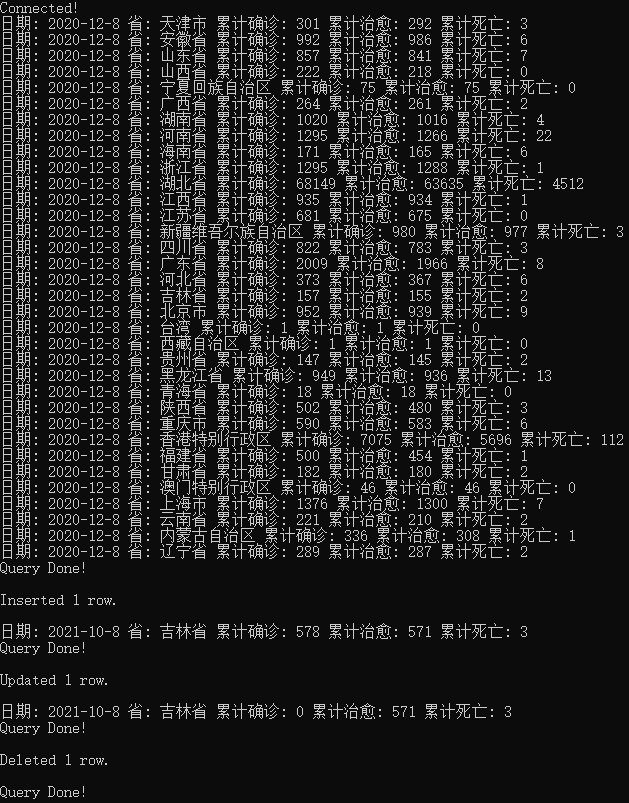
\includegraphics[width=0.7\linewidth]{./Images/running.png}
    \caption{运行截图\label{fig:running}}

\end{figure}

\section{测试结果}

\subsection{测试集1}

此测试集用于简单地测试程序是否正常运行。

\subsubsection{输入}

文法如\ref{grammar_text}节所示。

\begin{code}
    \begin{minted}{text}
num + num
\end{minted}
\end{code}

\subsubsection{输出}

\begin{code}
    \begin{minted}{text}
[Nonterminal Symbols] F T E 
[Terminal Symbols] * - ( num / ) + 
[Start Symbol] E
[Productions]
F -> ( E ) 
F -> num 
T -> T * F 
T -> T / F 
T -> F 
E -> E + T 
E -> E - T 
E -> T 

[Nonterminal Symbols] F T E' E 
[Terminal Symbols] * - ( num / ) + 
[Start Symbol] E'
[Productions]
F -> ( E ) 
F -> num 
T -> T * F 
T -> T / F 
T -> F 
E' -> E 
E -> E + T 
E -> E - T 
E -> T 

[DFA]
I0:
E' -> · E     $ 
E -> · E + T     + - $ 
E -> · E - T     + - $ 
E -> · T     + - $ 
T -> · T * F     $ - + / * 
T -> · T / F     $ - + / * 
T -> · F     $ - + / * 
F -> · ( E )     + / * - $ 
F -> · num     + / * - $ 
--- F --> I3
--- T --> I2
--- num --> I5
--- ( --> I4
--- E --> I1

I1:
E -> E · + T     - $ + 
E -> E · - T     - $ + 
E' -> E ·     $ 
--- - --> I7
--- + --> I6

I2:
T -> T · * F     * + / $ - 
T -> T · / F     * + / $ - 
E -> T ·     - $ + 
--- / --> I9
--- * --> I8

I3:
T -> F ·     * + / $ - 

I4:
E -> · E + T     - + ) 
E -> · E - T     - + ) 
E -> · T     - + ) 
T -> · T * F     ) - + / * 
T -> · T / F     ) - + / * 
T -> · F     ) - + / * 
F -> · ( E )     - + / * ) 
F -> ( · E )     - $ * + / 
F -> · num     - + / * ) 
--- F --> I12
--- T --> I11
--- num --> I14
--- ( --> I13
--- E --> I10

I5:
F -> num ·     - $ * + / 

I6:
E -> E + · T     $ - + 
T -> · T * F     $ - + / * 
T -> · T / F     $ - + / * 
T -> · F     $ - + / * 
F -> · ( E )     * $ - / + 
F -> · num     * $ - / + 
--- num --> I5
--- ( --> I4
--- F --> I3
--- T --> I15

I7:
E -> E - · T     $ - + 
T -> · T * F     $ - + / * 
T -> · T / F     $ - + / * 
T -> · F     $ - + / * 
F -> · ( E )     * $ - / + 
F -> · num     * $ - / + 
--- num --> I5
--- ( --> I4
--- F --> I3
--- T --> I16

I8:
T -> T * · F     * / + - $ 
F -> · ( E )     * / + - $ 
F -> · num     * / + - $ 
--- num --> I5
--- ( --> I4
--- F --> I17

I9:
T -> T / · F     * / + - $ 
F -> · ( E )     * / + - $ 
F -> · num     * / + - $ 
--- num --> I5
--- ( --> I4
--- F --> I18

I10:
E -> E · + T     ) + - 
E -> E · - T     ) + - 
F -> ( E · )     + / * - $ 
--- ) --> I21
--- - --> I20
--- + --> I19

I11:
T -> T · * F     * + / - ) 
T -> T · / F     * + / - ) 
E -> T ·     ) + - 
--- / --> I23
--- * --> I22

I12:
T -> F ·     * + / - ) 

I13:
E -> · E + T     - + ) 
E -> · E - T     - + ) 
E -> · T     - + ) 
T -> · T * F     ) - + / * 
T -> · T / F     ) - + / * 
T -> · F     ) - + / * 
F -> · ( E )     - + / * ) 
F -> ( · E )     ) * + / - 
F -> · num     - + / * ) 
--- F --> I12
--- T --> I11
--- num --> I14
--- ( --> I13
--- E --> I24

I14:
F -> num ·     ) * + / - 

I15:
T -> T · * F     * + / $ - 
T -> T · / F     * + / $ - 
E -> E + T ·     + $ - 
--- / --> I9
--- * --> I8

I16:
T -> T · * F     * + / $ - 
T -> T · / F     * + / $ - 
E -> E - T ·     + $ - 
--- / --> I9
--- * --> I8

I17:
T -> T * F ·     - $ / + * 

I18:
T -> T / F ·     - $ / + * 

I19:
E -> E + · T     + ) - 
T -> · T * F     + / ) - * 
T -> · T / F     + / ) - * 
T -> · F     + / ) - * 
F -> · ( E )     * / + ) - 
F -> · num     * / + ) - 
--- num --> I14
--- ( --> I13
--- F --> I12
--- T --> I25

I20:
E -> E - · T     + ) - 
T -> · T * F     + / ) - * 
T -> · T / F     + / ) - * 
T -> · F     + / ) - * 
F -> · ( E )     * / + ) - 
F -> · num     * / + ) - 
--- num --> I14
--- ( --> I13
--- F --> I12
--- T --> I26

I21:
F -> ( E ) ·     - $ * + / 

I22:
T -> T * · F     * / + - ) 
F -> · ( E )     * / + - ) 
F -> · num     * / + - ) 
--- num --> I14
--- ( --> I13
--- F --> I27

I23:
T -> T / · F     * / + - ) 
F -> · ( E )     * / + - ) 
F -> · num     * / + - ) 
--- num --> I14
--- ( --> I13
--- F --> I28

I24:
E -> E · + T     ) + - 
E -> E · - T     ) + - 
F -> ( E · )     - + / * ) 
--- ) --> I29
--- - --> I20
--- + --> I19

I25:
T -> T · * F     * - ) + / 
T -> T · / F     * - ) + / 
E -> E + T ·     - + ) 
--- / --> I23
--- * --> I22

I26:
T -> T · * F     * - ) + / 
T -> T · / F     * - ) + / 
E -> E - T ·     - + ) 
--- / --> I23
--- * --> I22

I27:
T -> T * F ·     ) - / + * 

I28:
T -> T / F ·     ) - / + * 

I29:
F -> ( E ) ·     ) * + / - 


[Parsing Table]
State 0
    Nonterminal    (
    Action         S 4
    Nonterminal    num
    Action         S 5
    Terminal       E
    Goto           1
    Terminal       T
    Goto           2
    Terminal       F
    Goto           3
State 1
    Nonterminal    +
    Action         S 6
    Nonterminal    $
    Action         ACC
    Nonterminal    -
    Action         S 7
State 2
    Nonterminal    $
    Action         R E -> T 
    Nonterminal    -
    Action         R E -> T 
    Nonterminal    *
    Action         S 8
    Nonterminal    +
    Action         R E -> T 
    Nonterminal    /
    Action         S 9
State 3
    Nonterminal    -
    Action         R T -> F 
    Nonterminal    $
    Action         R T -> F 
    Nonterminal    /
    Action         R T -> F 
    Nonterminal    +
    Action         R T -> F 
    Nonterminal    *
    Action         R T -> F 
State 4
    Nonterminal    (
    Action         S 13
    Nonterminal    num
    Action         S 14
    Terminal       E
    Goto           10
    Terminal       T
    Goto           11
    Terminal       F
    Goto           12
State 5
    Nonterminal    /
    Action         R F -> num 
    Nonterminal    +
    Action         R F -> num 
    Nonterminal    *
    Action         R F -> num 
    Nonterminal    $
    Action         R F -> num 
    Nonterminal    -
    Action         R F -> num 
State 6
    Nonterminal    (
    Action         S 4
    Nonterminal    num
    Action         S 5
    Terminal       T
    Goto           15
    Terminal       F
    Goto           3
State 7
    Nonterminal    (
    Action         S 4
    Nonterminal    num
    Action         S 5
    Terminal       T
    Goto           16
    Terminal       F
    Goto           3
State 8
    Nonterminal    (
    Action         S 4
    Nonterminal    num
    Action         S 5
    Terminal       F
    Goto           17
State 9
    Nonterminal    (
    Action         S 4
    Nonterminal    num
    Action         S 5
    Terminal       F
    Goto           18
State 10
    Nonterminal    +
    Action         S 19
    Nonterminal    -
    Action         S 20
    Nonterminal    )
    Action         S 21
State 11
    Nonterminal    -
    Action         R E -> T 
    Nonterminal    )
    Action         R E -> T 
    Nonterminal    *
    Action         S 22
    Nonterminal    +
    Action         R E -> T 
    Nonterminal    /
    Action         S 23
State 12
    Nonterminal    )
    Action         R T -> F 
    Nonterminal    -
    Action         R T -> F 
    Nonterminal    /
    Action         R T -> F 
    Nonterminal    +
    Action         R T -> F 
    Nonterminal    *
    Action         R T -> F 
State 13
    Nonterminal    (
    Action         S 13
    Nonterminal    num
    Action         S 14
    Terminal       E
    Goto           24
    Terminal       T
    Goto           11
    Terminal       F
    Goto           12
State 14
    Nonterminal    -
    Action         R F -> num 
    Nonterminal    /
    Action         R F -> num 
    Nonterminal    +
    Action         R F -> num 
    Nonterminal    *
    Action         R F -> num 
    Nonterminal    )
    Action         R F -> num 
State 15
    Nonterminal    -
    Action         R E -> E + T 
    Nonterminal    $
    Action         R E -> E + T 
    Nonterminal    *
    Action         S 8
    Nonterminal    +
    Action         R E -> E + T 
    Nonterminal    /
    Action         S 9
State 16
    Nonterminal    -
    Action         R E -> E - T 
    Nonterminal    $
    Action         R E -> E - T 
    Nonterminal    *
    Action         S 8
    Nonterminal    +
    Action         R E -> E - T 
    Nonterminal    /
    Action         S 9
State 17
    Nonterminal    *
    Action         R T -> T * F 
    Nonterminal    +
    Action         R T -> T * F 
    Nonterminal    /
    Action         R T -> T * F 
    Nonterminal    $
    Action         R T -> T * F 
    Nonterminal    -
    Action         R T -> T * F 
State 18
    Nonterminal    *
    Action         R T -> T / F 
    Nonterminal    +
    Action         R T -> T / F 
    Nonterminal    /
    Action         R T -> T / F 
    Nonterminal    $
    Action         R T -> T / F 
    Nonterminal    -
    Action         R T -> T / F 
State 19
    Nonterminal    (
    Action         S 13
    Nonterminal    num
    Action         S 14
    Terminal       T
    Goto           25
    Terminal       F
    Goto           12
State 20
    Nonterminal    (
    Action         S 13
    Nonterminal    num
    Action         S 14
    Terminal       T
    Goto           26
    Terminal       F
    Goto           12
State 21
    Nonterminal    /
    Action         R F -> ( E ) 
    Nonterminal    +
    Action         R F -> ( E ) 
    Nonterminal    *
    Action         R F -> ( E ) 
    Nonterminal    $
    Action         R F -> ( E ) 
    Nonterminal    -
    Action         R F -> ( E ) 
State 22
    Nonterminal    (
    Action         S 13
    Nonterminal    num
    Action         S 14
    Terminal       F
    Goto           27
State 23
    Nonterminal    (
    Action         S 13
    Nonterminal    num
    Action         S 14
    Terminal       F
    Goto           28
State 24
    Nonterminal    +
    Action         S 19
    Nonterminal    -
    Action         S 20
    Nonterminal    )
    Action         S 29
State 25
    Nonterminal    )
    Action         R E -> E + T 
    Nonterminal    -
    Action         R E -> E + T 
    Nonterminal    *
    Action         S 22
    Nonterminal    +
    Action         R E -> E + T 
    Nonterminal    /
    Action         S 23
State 26
    Nonterminal    )
    Action         R E -> E - T 
    Nonterminal    -
    Action         R E -> E - T 
    Nonterminal    *
    Action         S 22
    Nonterminal    +
    Action         R E -> E - T 
    Nonterminal    /
    Action         S 23
State 27
    Nonterminal    *
    Action         R T -> T * F 
    Nonterminal    +
    Action         R T -> T * F 
    Nonterminal    /
    Action         R T -> T * F 
    Nonterminal    -
    Action         R T -> T * F 
    Nonterminal    )
    Action         R T -> T * F 
State 28
    Nonterminal    *
    Action         R T -> T / F 
    Nonterminal    +
    Action         R T -> T / F 
    Nonterminal    /
    Action         R T -> T / F 
    Nonterminal    -
    Action         R T -> T / F 
    Nonterminal    )
    Action         R T -> T / F 
State 29
    Nonterminal    -
    Action         R F -> ( E ) 
    Nonterminal    /
    Action         R F -> ( E ) 
    Nonterminal    +
    Action         R F -> ( E ) 
    Nonterminal    *
    Action         R F -> ( E ) 
    Nonterminal    )
    Action         R F -> ( E ) 

Stack
0   
$   
Input          num + num $ 
Output         Shift 5

Stack
0   5   
$   num 
Input          + num $ 
Output         Reduce by F -> num 

Stack
0   3   
$   F   
Input          + num $ 
Output         Reduce by T -> F 

Stack
0   2   
$   T   
Input          + num $ 
Output         Reduce by E -> T 

Stack
0   1   
$   E   
Input          + num $ 
Output         Shift 6

Stack
0   1   6   
$   E   +   
Input          num $ 
Output         Shift 5

Stack
0   1   6   5   
$   E   +   num 
Input          $ 
Output         Reduce by F -> num 

Stack
0   1   6   3   
$   E   +   F   
Input          $ 
Output         Reduce by T -> F 

Stack
0   1   6   15  
$   E   +   T   
Input          $ 
Output         Reduce by E -> E + T 

Stack
0   1   
$   E   
Input          $ 
Output         Accepted!

Parsing successful!
\end{minted}
\end{code}

\subsubsection{分析}

程序首先输出原文法,之后输出拓广文法、识别所有活前缀的DFA、预测分析表。最后程序给出了分析字符串的过程。

\subsection{测试集2}

此测试集测试一个复杂的算术表达式。

\subsubsection{输入}

文法如\ref{grammar_text}节所示。

\begin{code}
    \begin{minted}{text}
( num * ( ( ( ( num + num ) * num ) + num / num ) - num * ( num + num ) ) / num )
\end{minted}
\end{code}

\subsubsection{输出}

由于输出内容过长,不在此展开,请参考\href{run:../test/result2.txt}{输出文件}。

\subsubsection{分析}

正确分析了此字符串。

\subsection{测试集3}

此测试集用于测试一个错误的算术表达式。

\subsubsection{输入}

文法如\ref{grammar_text}节所示。

\begin{code}
    \begin{minted}{text}
( num + num ) * / num
\end{minted}
\end{code}

\subsubsection{输出}

由于输出内容过长,不在此展开,请参考\href{run:../test/result3.txt}{输出文件}。

\subsubsection{分析}

归约到\mintinline{text}{T*}时,无法再进行归约,分析程序报错并退出。

\subsection{测试集4}

此测试集用于测试一个错误的算术表达式。

\subsubsection{输入}

文法如\ref{grammar_text}节所示。

\begin{code}
    \begin{minted}{text}
( ( num + num ) / num
\end{minted}
\end{code}

\subsubsection{输出}

由于输出内容过长,不在此展开,请参考\href{run:../test/result4.txt}{输出文件}。

\subsubsection{分析}

归约到\mintinline{text}{(T/num}时,无法再进行归约,分析程序报错并退出。

\subsection{测试集5}

此测试集依照习题4.10修改而来。

\subsubsection{输入}

\begin{code}
    \begin{minted}{text}
$ Nonterminal symbols
E L
$ Terminal symbols
a , ( )
$ Start symbol
E
$ Productions
E -> ( L ) $ a
L -> L , E $ E
\end{minted}
\end{code}

\begin{code}
    \begin{minted}{text}
( ( a ) , a , ( a , a ) )
\end{minted}
\end{code}

\subsubsection{输出}

由于输出内容过长,不在此展开,请参考\href{run:../test/result5.txt}{输出文件}。

\subsection{测试集6}

此测试集依照习题4.18修改而来。

\subsubsection{输入}

\begin{code}
    \begin{minted}{text}
$ Nonterminal symbols
S A B
$ Terminal symbols
a b
$ Start symbol
S
$ Productions
S -> A
A -> B A $ [empty]
B -> a B $ b
\end{minted}
\end{code}

\begin{code}
    \begin{minted}{text}
a b a b
\end{minted}
\end{code}

\subsubsection{输出}

由于输出内容过长,不在此展开,请参考\href{run:../test/result6.txt}{输出文件}。

\section{实验总结}

本次实验中我编写了一个LR(1)语法分析程序,使我对自底向上语法分析的流程更加清楚,对相关知识点的掌握更加牢固。

此程序的架构比较简单,主要难点在数据结构的设计和算法的实现方面,尤其是对于LR(1)项目和项目集,表示方式需要既准确又要便于计算,实现的难度较大。
在实现期间,我使用了C++11的语法特性,使得算法过程更加清晰,大大减少编程复杂度。

在成功实现这些算法并且通过测试之后,我尝试编写了伪代码,这将会为我未来解题带来很大帮助。

此外,我的语法分析程序仍然存在许多待改进的地方,比如对于对于错误的处理不够全面、在求解DFA时的鲁棒性仍然有待提高,由于时间所限,这些情况我无法一一考虑周全。

本次实验除了让我对课内知识有了更多的认识,也使我的C++编程能力得到提高,我从中收获颇丰。

\end{document}